%%%%%%%%%%%%%%%%%%%%%%%%%%%%%%%%%%%%%%%%%%%%%%%%%%%%%%%%%%%%%%%%%%%
%                                                                 %
%                            CHAPTER THREE                        %
%                                                                 %
%%%%%%%%%%%%%%%%%%%%%%%%%%%%%%%%%%%%%%%%%%%%%%%%%%%%%%%%%%%%%%%%%%%

\chapter{CAVITY-BASED CONFORMAL MESH ADAPTATION}
\label{chap:adapt}

\section{In Context}

The mesh adaptation methods in this work are both
conformal, general, and cavity-based.
They are conformal in the sense that the boundaries of all
elements (Section \ref{sec:def_complex}) are composed
of the set of entities expected by that element's
topological template (Section \ref{sec:topo_template}).
In other words, we avoid the ``hanging node" scenarios
introduced by non-conformal mesh modification techniques.
Typically, non-conformal mesh modification also restricts
itself to subdividing input elements into more elements,
or undoing such subdivisions which were done before.
Figure \ref{fig:hex_amr} illustrates such a method,
and clearly shows the hanging nodes introduced.

\begin{figure}
\begin{center}
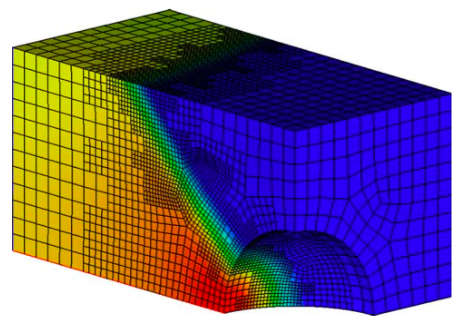
\includegraphics[width=0.6\textwidth]{hex_amr.png}
\caption{Non-conforming parent-child adaptive mesh refinement
\cite{kirk2006libmesh}}
\label{fig:hex_amr}
\end{center}
\end{figure}

Non-conforming meshes require additional support from
the PDE-solving code to deal with hanging nodes, and typically
no more than one level of refinement is allowed between adjacent
elements.
The more important limitation is due to non-conforming methods
typically being parent-child methods, which fundamentally limits
them to the topology of the coarse input mesh.
If this input mesh is more fine than necessary in some areas,
it cannot be coarsened.
If moving objects or object deformation cause input elements
to become highly compressed or even inverted, parent-child
refinement can never correct or prevent this.
For these reasons we take a general approach, employing
coarsening, swapping, and possibly other operations which are
able to coarsen beyond the input mesh and correct low-quality
elements in the input mesh.

We restrict ourselves to local cavity operations as well,
meaning that the transformation from input to output meshes
can be expressed as a series of cavity modifications, each
of which can in turn be expressed as a the removal of
a small number of mesh entities followed by the addition
of a small number of mesh entities.
In this case small means a number which can be bounded
by a constant and is not affected by the total number
of mesh entities.

The benefits of using local cavity operations are:
\begin{enumerate}
\item It allows more straightforward and reliable parallelization of
mesh adaptation (see Section \ref{sec:cavity_sched}).
\item It allows much more careful control of the effects that mesh
adaptation has on the simulation fields attached to the mesh.
\end{enumerate}

On the other hand, the set of known cavity operations
have been found by the trial and error of researchers,
and there are many properties which they are not guaranteed to
achieve.
The most successful set of cavity operators are those
which operate on simplex meshes, due ultimately to the
fact that a simplex is the simplest polytope of a given dimension,
and that more complex polytopes require exponentially more
complex considerations.
In our work, we separate cavity operators into three categories:
\begin{enumerate}
\item Refinement: create a strictly more detailed discretization
than the input. Guaranteed not to invert elements, but not to
preserve any element quality. Guaranteed to exactly preserve
the distribution of fields.
\item Coarsening: create a strictly less detailed discretization
than the input. No guarantees it can be done without reducing
or negating quality, so it must be checked.
By definition, cannot exactly preserve the distribution of the fields.
\item Shape correction: typically maintains similar level of detail,
modifies connectivity to improve minimum element quality.
There is no known method guaranteed to raise all elements to a quality
that is useful for simulation and adaptation, but heuristic
methods can achieve great results in practice \cite{klingner2008aggressive}.
\end{enumerate}

\section{Related Work}

There have been several iterations of the MeshAdapt
library developed at RPI.
One of the earliest publications by De Cougny and Shephard
\cite{de1999parallel} outlines the three basic steps and goes into some detail
on a use of independent sets for coarsening purposes
(an idea that we extend significantly in Section \ref{sec:indset}.
Later, much work was done by Li on anisotropy using the metric
tensor and the selection of operators for shape correction
\cite{li20053d,li2003mesh}.
Our implementations of tetrahedral edge swaps make use
of guidance on fast implementation by Olivier-Gooch \cite{freitag1997tetrahedral}.
Researchers at INRIA have provided useful mathematical foundations
for handling the anisotropic metric tensor field
\cite{frey2005,alauzet2006parallel,loseille2015parallel},
and work at the Catholic University of Louvain explored
the use of mesh adaptation to respond to moving objects
\cite{compere2010mesh}, a path we continue with our Omega\_h work.

\section{MeshAdapt Methods}
\label{sec:ma_methods}

\subsection{Template Refinement}

The MeshAdapt library uses edge-based refinement templates for its refinement step.
The way these work is that all edges whose metric length exceeds some threshold
$l_{\text{up}} > 1$ are marked for refinement.
Then each element takes into account the subset of its edges which are marked
for refinement, and chooses one of many possible subdivision patterns
(refinement templates) based on this subset of edges.
Figure \ref{fig:tet_templates} illustrates these templates in the case of tetrahedra.
In fact, the center template shown for three marked edges has two variants which
are symmetric by reflection but not by rotation.
In total, this means there are 12 rotationally unique tetrahedron refinement templates.

\begin{figure}
\begin{center}
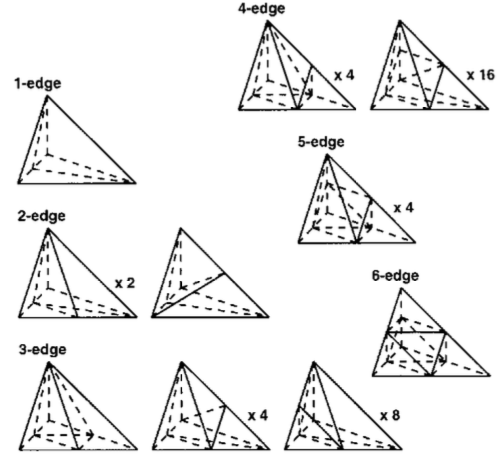
\includegraphics[width=0.6\textwidth]{tet_templates.png}
\caption{Tetrahedral refinement templates}
\label{fig:tet_templates}
\end{center}
\end{figure}

One benefit of the use of refinement templates is that adjacent elements can be refined
simultaneously, so all edges, faces, and regions of the mesh can be modified in
a nearly embarrassingly parallel fashion once the set of marked edges is identified.
Another benefit is that the gradation of the mesh is more explicitly controlled
compared to methods which split edges independently.
However, refinement templates have some drawbacks as well:
\begin{enumerate}
\item In some cases, a subset of the template is a polyhedron that cannot be
subdivided into tetrahedra without introducing an extra vertex within the
parent tetrahedron.
In particular, Sch{\"o}nhardt's polyhedron can appear (see Figure
\ref{fig:schonhardt}).
This reduces the predictability of refinement and makes it more difficult
to transfer solution.
\item Other cases introduce a geometric decision, such as the case
when all edges of a tetrahedron are refined, or even when two edges
of a triangle are refined. This also reduces predictability.
\item It takes substantial code to implement all rotationally unique
combinations for all the relevant element polytopes.
This increases the likelihood of errors and decreases the productivity
of modifying any aspect of refinement.
\item Due to the simultaneous nature of the operation and the difficulty
of predicting the outcome, it is prohibitively difficult to reject
a local portion of the refinement based on criteria such as new elements
having too low quality.
\end{enumerate}

\begin{figure}
\begin{center}
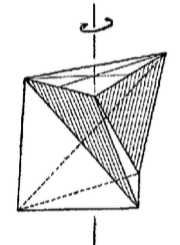
\includegraphics[width=0.2\textwidth]{schonhardt.png}
\caption{Sch{\"o}nhardt's irreducible polyhedron
\cite{Schonhardt1928}}
\label{fig:schonhardt}
\end{center}
\end{figure}

\subsection{Coarsening}

Like other adaptation libraries, MeshAdapt implements
coarsening via edge collapses.
Figure \ref{fig:collapse} shows a typical edge collapse
in a tetrahedral mesh for reference.
One vertex in the mesh is ``moved" onto another vertex which is adjacent
via a mesh edge, collapsing this edge and all its adjacent
faces and regions.
For programming purposes, when dealing with sets of entities we
can call those being removed the ``collapsing" set and those being
conceptually elongated to fill the cavity as the set to ``keep".
In practice all old entities are removed and the set of entities to keep
is rebuilt with modified connectivity (where they were adjacent to the
collapsed vertex, now they are adjacent to the kept vertex, etc).

\begin{figure}
\begin{center}
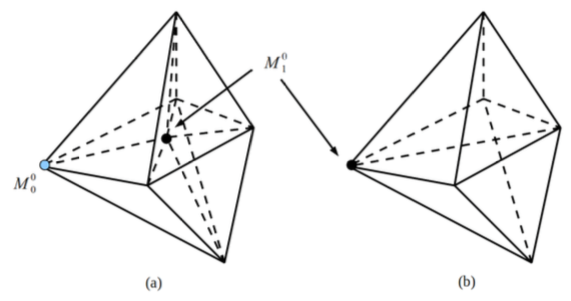
\includegraphics[width=0.6\textwidth]{collapse.png}
\caption{Edge collapse in tetrahedral mesh
\cite{lu2011developments}}
\label{fig:collapse}
\end{center}
\end{figure}

Edge collapsing is an operation which, if not properly controlled,
can invalidate the mesh topologically or undo its topological similarity
to a CAD model.
MeshAdapt uses a set of checks which is somewhat expensive to compute
but is quite topologically robust:

\begin{enumerate}
\item The vertex being collapsed must have the same classification as
the edge being collapsed. This preserves similarity to the CAD model by
preventing collapses from the boundary into the interior.
\item If there exists a ring of three edges including the collapsing edge
(Figure \ref{fig:edge_ring}),
then those three edges must bound a single triangle in the mesh.
This prevents collapsing an empty hole in the mesh to zero volume,
see Figure \ref{fig:circle_hole}.
In addition, the non-collapsing edge adjacent to the collapsing vertex must have the same
classification as this triangle.
This prevents collapsing a cavity on a curved boundary down to zero volume
(see Figure \ref{fig:surf_collapse}), which would require re-classifying
entities on the cavity boundary (which breaks parallelism guarantees), and
create no elements in the new cavity (which is problematic for solution transfer).
\item Analogous to the edge ring check, in 3D we check for two triangles which
share a non-collapsing edge and whose remaining two vertices are the endpoints
of the collapsing edge.
The two triangles and the collapsing edge must bound a single tetrahedron,
and the triangle adjacent to the collapsing vertex must have the same classification
as this tetrahedron.
\end{enumerate}

\begin{figure}
\begin{center}
\includegraphics[width=0.6\textwidth]{edge_ring.png}
\caption{Edge ring condition check during edge collapse}
\label{fig:edge_ring}
\end{center}
\end{figure}

\subsection{Shape Correction}

\begin{figure}
\begin{center}
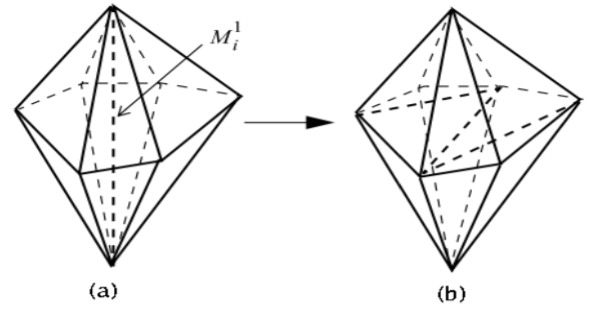
\includegraphics[width=0.6\textwidth]{swap.png}
\caption{Edge swap in tetrahedral mesh
\cite{lu2011developments}}
\label{fig:swap}
\end{center}
\end{figure}

\begin{figure}
\begin{center}
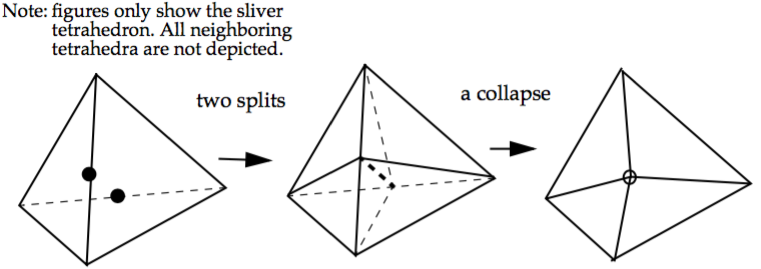
\includegraphics[width=0.6\textwidth]{split_collapse.png}
\caption{Double-split + collapse compound operator
\cite{li2003mesh}}
\label{fig:compound}
\end{center}
\end{figure}

\section{Omega\_h Methods}
\label{sec:omega_h-adapt}

Focuses on serial aspects, i.e. single splits and
quality restrictions.

\section{Size Field Algorithms}
\label{sec:sf}

\subsection{Metric Storage and Interpolation}

The metric tensor field introduced in Section \ref{sec:def_metric}
is typically provided as a set of values defined at mesh vertices.
This leads to an important question about how to compute metric
tensor values at other points in the mesh, i.e. how to interpolate
the metric tensor.
We can illustrate the issues involved with the simplest interpolation
case, that of deriving a metric tensor for the center of a mesh
edge given the two metric tensors at its endpoints.
Unfortunately, linear interpolation of the components of the
tensor $\mathcal{M}$ itself has the undesirable property that
interpolating between two highly anisotropic metrics of even
slightly different orientations will tend to produce isotropic
results with very small desired lengths, i.e. the longer desired
length will be lost.
For this reason, alternative interpolation methods have been developed
focusing on getting desired results in the case of high anisotropy.
Some of the most relevant are as follows:

\begin{enumerate}
\item MeshAdapt works with an internal representation consisting
of the orthogonal matrix $R$ and the vector of desired lengths
$\mathbf{h} = (h_1, h_2, h_3)^T$ which form the metric tensor:
\begin{equation}
\mathcal{M} = R^T \begin{bmatrix}
1 / h_1 & 0 & 0 \\
0 & 1 / h_2 & 0 \\
0 & 0 & 1 / h_3 \\
\end{bmatrix} R
\end{equation}
Each of these is then interpolated separately.
The vector $\mathbf{h}$ is linearly interpolated, while the
matrix $R$ is first linearly interpolated, and then re-orthogonalized
using the Gram-Schmidt process.
The benefit of this is that anisotropy is fully preserved due to the
separate interpolation of lengths.
However, there are three main drawbacks to this method:
\begin{enumerate}
\item The interpolation of $R$ is fragile, because if the linearly
interpolated value is rank-deficient then re-orthogonalization
will fail. This can happen, for example, if the two input $R$ matrices
represent rotations that are $180^{\circ}$ away from each other.
Even though these represent exactly the same metric tensor, interpolation
would fail.
\item The overall method gives results which depend too much on the
details of how the tensor was decomposed.
If we have two metrics which are $90^{\circ}$ away from each other
as shown in Figure \ref{fig:90deg_interp},
their interpolated result depends heavily on the signs of the eigenvectors
chosen for $R$.
\item This method stores 12 components per vertex on a 3D mesh, whereas
the alternatives below store only 6.
\end{enumerate}
\item Omega\_h computes the inverse of the metric tensors, then
interpolates those linearly, and inverts the result.
This is a method proposed by Alauzet and Frey as a compromise between
the anisotropic fidelity and high runtime costs of the following two methods
\cite{alauzet2003estimateur}.
\item The highest fidelity interpolation suggested by Alauzet and Frey is
the Power method which linearly interpolate $\mathcal{M}^{-1/2}$,
which equals $\mathcal{M}$ replacing each eigenvalue $\lambda$
with $(1/\sqrt{\lambda})$.
This requires the additional expense of computing an eigendecomposition.
\item An even better fidelity interpolation suggested by Loseille and
L{\"o}hner \cite{loseille20093d} and later confirmed by
Michal and Krakos \cite{michal2012anisotropic} is the Log-Euclidean
method which linearly interpolates $\log(\mathcal{M})$, which equals
$\mathcal{M}$ replacing the eigenvalues $\lambda$ with $\log(\lambda)$.
Figure \ref{fig:log_interp} shows how this method better preserves
very high levels of anisotropy.
\end{enumerate}

\begin{figure}
\begin{center}
\includegraphics[width=0.6\textwidth]{90deg_interp.png}
\caption{MeshAdapt interpolation depends on eigenvector signs}
\label{fig:90deg_interp}
\end{center}
\end{figure}

\begin{figure}
\begin{center}
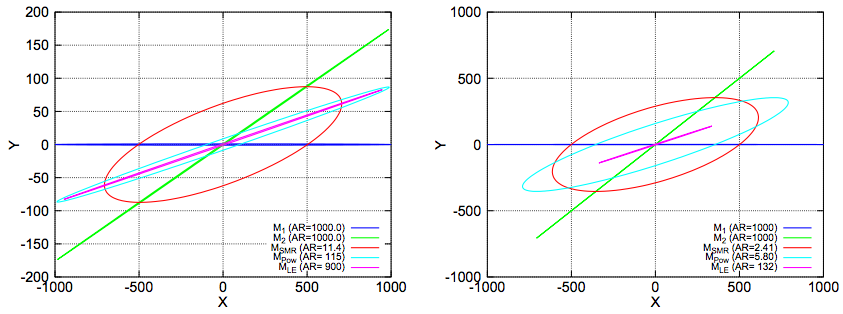
\includegraphics[width=0.95\textwidth]{log_interp.png}
\caption{Log-Euclidean versus Power interpolation
at 1:1000 anisotropy
\cite{michal2012anisotropic}}
\label{fig:log_interp}
\end{center}
\end{figure}

To date the former two methods have proved sufficient for varying
degrees of anisotropy, yet we consider the implementation of one
of the latter two methods as an area of immediate future work.

\subsection{Identity Size Field}

\subsection{Targeting an Element Count}

\section{Solution Transfer in a Cavity}

Emphasize numerical / performance advantage
over full-mesh methods.
Results can be included for each particular
method if it warrants one.

\subsection{Conserving Integral Quantities}

\section{Serial Adaptation Performance}

Both absolute performance and perhaps comparing
different methods.

%%% Local Variables:
%%% mode: latex
%%% TeX-master: t
%%% End:


